% !TEX TS-program = pdflatex
% !TeX encoding = UTF-8
% !TeX spellcheck = en_GB

\documentclass[aspectratio=43]{beamer}
% use this instead for 16:9 aspect ratio:
%\documentclass[aspectratio=169]{beamer}
% supported acpect ratios  1610  169 149 54 43 (deault) 32
%

\usepackage[english]{babel} 
\usepackage[utf8]{inputenc}
\usepackage[T1]{fontenc} 	
\usetheme{ETHbeamer}

\colorlet{ETHcolor1}{ETHc}
\colorlet{ETHcolor2}{ETHi}

\author{Jonathan Maurer, Jonathan Rosenthal, Jonas Kuratli}

\title{Design of a Parallel Chess Engine}

\date{2016-11-07}

% uncomment if you do not want to use a department logo
\deplogofalse


\begin{document}

\titleframe

\setbeamerfont{footnote}{size=\tiny}



\begin{frame}
\frametitle{Simple Approach}

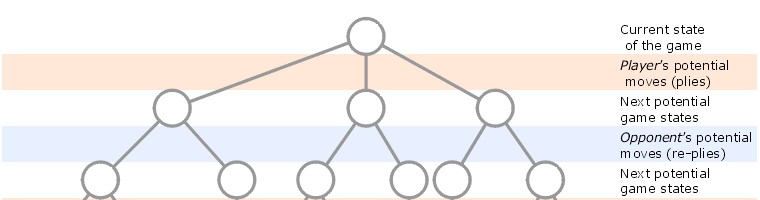
\includegraphics[width=\textwidth]{tree}

\footnotetext{Picture from English Language Wikipedia, https://en.wikipedia.org/wiki/File:Minmaxab.gif}


\end{frame}

\begin{frame}
\frametitle{Simple Approach}

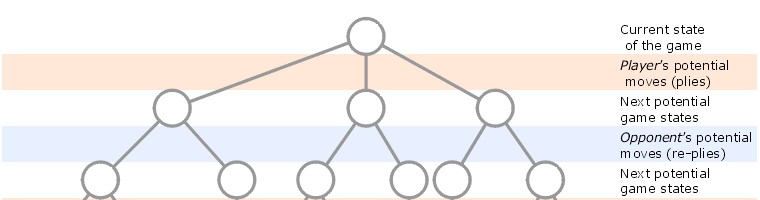
\includegraphics[width=\textwidth]{tree}

\begin{itemize}
\item Evaluate states up to a pre-defined depth d bottom-up
\item Leaf evaluated using an evaluation function
\item Other nodes evaluated by finding min or max of children

\end{itemize}

\footnotetext{Picture from English Language Wikipedia, https://en.wikipedia.org/wiki/File:Minmaxab.gif}
\end{frame}

\begin{frame}
\frametitle{Simple Approach}

Pros:
\begin{itemize}
\item Easy to implement
\item Easy to parallelize (Distribute evaluation of children)
\end{itemize}

Cons:
\begin{itemize}
\item Tree becomes broad very quickly 
\item Message passing overhead if parallelized
\end{itemize}
\end{frame}

\begin{frame}
\frametitle{Alpha-Beta Pruning}
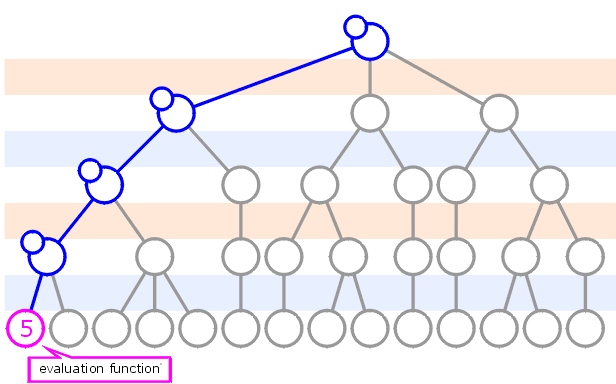
\includegraphics[width=\textwidth]{alpha1}
\footnotetext{Picture from English Language Wikipedia, https://en.wikipedia.org/wiki/File:Minmaxab.gif}
\end{frame}

\begin{frame}
\frametitle{Alpha-Beta Pruning}
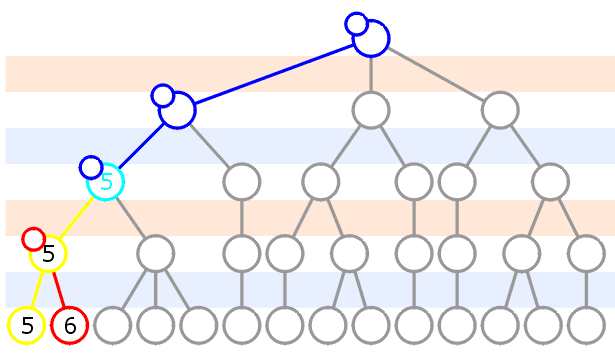
\includegraphics[width=\textwidth]{alpha2}
\footnotetext{Picture from English Language Wikipedia, https://en.wikipedia.org/wiki/File:Minmaxab.gif}
\end{frame}

\begin{frame}
\frametitle{Alpha-Beta Pruning}
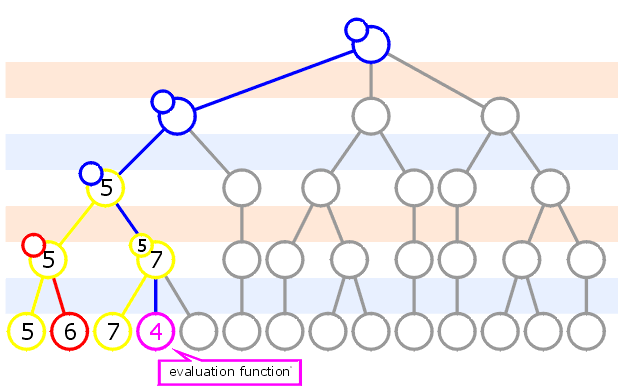
\includegraphics[width=\textwidth]{alpha3}
\footnotetext{Picture from English Language Wikipedia, https://en.wikipedia.org/wiki/File:Minmaxab.gif}
\end{frame}

\begin{frame}
\frametitle{Alpha-Beta Pruning}
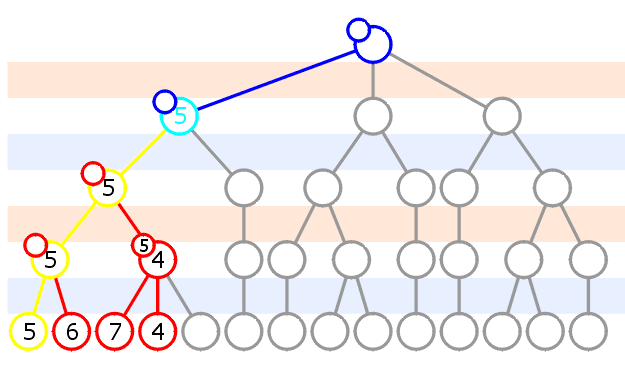
\includegraphics[width=\textwidth]{alpha4}
\footnotetext{Picture from English Language Wikipedia, https://en.wikipedia.org/wiki/File:Minmaxab.gif}
\end{frame}

\begin{frame}
\frametitle{Alpha-Beta Pruning}
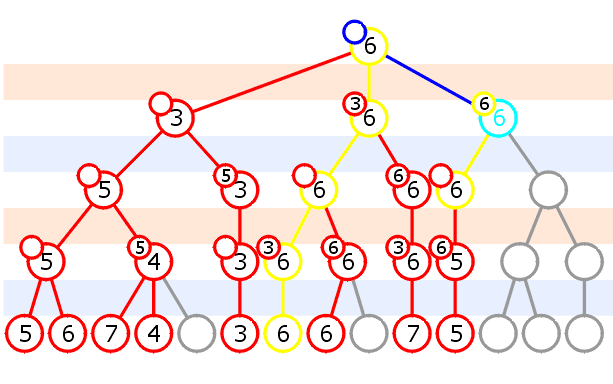
\includegraphics[width=\textwidth]{alpha5}
\footnotetext{Picture from English Language Wikipedia, https://en.wikipedia.org/wiki/File:Minmaxab.gif}
\end{frame}

\begin{frame}
\frametitle{Alpha-Beta Pruning}
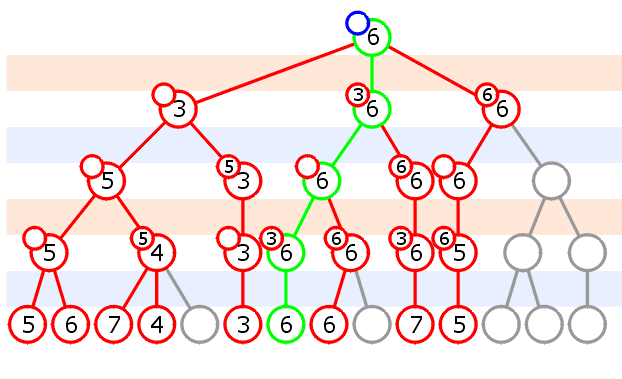
\includegraphics[width=\textwidth]{alpha6}
\footnotetext{Picture from English Language Wikipedia, https://en.wikipedia.org/wiki/File:Minmaxab.gif}
\end{frame}

\begin{frame}
\frametitle{Alpha-Beta Pruning}
Pros:
\begin{itemize}
\item Reduces \# of visited nodes
\end{itemize}

Cons:
\begin{itemize}
\item Harder to parallelize (Message propagation top-down AND bottom-up)
\end{itemize}
\end{frame}

\begin{frame}
\frametitle{Parallel Alpha-Beta Pruning}
Rough Plan:
\begin{itemize}
\item Parallel evaluation of nodes at a certain depth
\item Cut nodes with significantly worse evaluation than best node
\item Evaluate nodes ordered by evaluation value
\item Allocate resources by value
\end{itemize}
\end{frame}

\begin{frame}
\frametitle{Parallel Alpha-Beta Pruning}
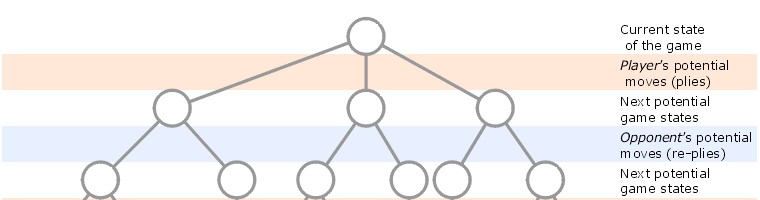
\includegraphics[width=\textwidth]{tree}
\footnotetext{Picture from English Language Wikipedia, https://en.wikipedia.org/wiki/File:Minmaxab.gif}
\end{frame}

\begin{frame}
\frametitle{Goals}

\begin{itemize}
\item Serial version of both approaches
\item Parallelize both appraoches
\item Determine gain from parallelization
\item Compare approaches depending on resources
\item Compare our approaches with existing ones
\end{itemize}
\end{frame}

\begin{frame}
\frametitle{Existing Work}
\begin{itemize}
\item First parallel engine was less efficient than its serial version
\item By 2013, 2 out of top 3 engines ran in parallel
\item By now, almost no top engines run serial implementation
\end{itemize}
\end{frame}

\begin{frame}
\frametitle{Current state}
\begin{itemize}
\item Serial versions of both approaches exist
\item Depth considered dependent on time remaining
\item Demonstration coming up...
\end{itemize}
\end{frame}



\end{document}
